\documentclass[a4paper]{jpconf}
\usepackage{graphicx}
\usepackage{html}
\begin{document}
\title{Designing Computing System Architecture and Models for the HL-LHC era}

\author{Stephen Gowdy}

\address{Fermilab, Batavia IL, USA}

\ead{sgowdy+chep15@gmail.com}

\begin{abstract}
This paper described the aims and objectives of a programme to study
the computing model in CMS after the next long shutdown near the end
of the decade.
\end{abstract}

\section{Introduction}

One of the recurring challenges for HEP computing in recent years
has been data management, access and organization when using
distributed computing resources.  The computing model chosen by CMS
for the LHC startup used a distributed data management
architecture~\cite{CMSCTDR} which placed datasets statically at
sites. Dataset replicas in multiple sites were made manually as
required, and jobs were sent to sites where their input data could
be read from site-local storage.  In the first years of the Worldwide
LHC Computing Grid (WLCG) many of the computer centers were new and
not yet operating at full reliability. The static placement strategy
minimized dependencies between centers and allowed for efficient
and scalable commissioning of the resources.  It had however the
disadvantage of requiring significantly more storage than strictly
necessary due to the dataset replication. The wide area network
(WAN) was also underutilized as a resource, despite being significantly
more robust than originally imagined.

The reliability of all WLCG computer centers has greatly improved
through the experience gained during LHC Run 1. More sophisticated
data management and access models are thus possible. A first step
in this direction is well underway. Via the NSF-funded ``Any Data,
Any Time, Anywhere'' (AAA) project, US-CMS currently leads an effort
to deploy a worldwide data federation~\cite{AAACHEP13}.  %based on
the xrootd data access system~\cite{XROOTD1}.  Via the data federation
an application running in one center can open a file for reading,
and the system will find and allow remote reads from a copy of the
file wherever it is located in the world. Efficient remote access
to data removes compute and storage locality requirements, and
permits reduction of extra storage costs resulting from dataset
replications.  The use of ``opportunistic'' compute resources also
becomes much easier, as they can be used without requiring local
data storage.  For LHC Run 2 CMS is deploying additional technologies
to monitor dataset popularity and use PhEDEx~\cite{PHEDEX} to remove
unnecessary dataset replications. These evolutionary changes will
allow effective data management and access through Run 2.

\section{Data Management at the HL-LHC}
Planning is currently underway for a High Luminosity Large Hadron
Collider (HL-LHC)~\cite{HLLHC} with an objective of accumulating
${3000fb^{-1}}$ by 2030. Taking into account the upcoming increase
in energy for Run 2, and expectations for evolving pile-up and
trigger rate through Run 3 and HL-LHC, the data volume increase
over the next 15 years will be O($10^3$).

Storage technologies are also evolving~\cite{SMSTORAGE}.  Disk size
growth per unit cost appears to be slowing. Access rates per unit
cost are stagnant and it isn't yet clear that the cost of SSD's
will drop enough to be a cost-effective replacement for disks at
very high storage volumes. Tape will however remain relatively
cheap. Simultaneously processor technology evolution towards
multi-core and many-core technologies~\cite{SMPROC} could change
significantly the I/O requirements of individual jobs. Trends towards
the use of diverse cloud-provisioned compute and storage
resources~\cite{SMEFCOMP} further motivate a more flexible and
dynamic data management.

Together these factors imply that HL-LHC (and perhaps Run 3) will
require larger, potentially non-evolutionary, changes to the
experiment's computing model, data management, access and organization.
To that end, a number of ideas and research questions have arisen
in the community: Can the architectures and algorithms used for
caching and to reduce latencies in Content Delivery Networks be
applied to building such a system?  What can be learned from
commercial/general purpose cloud storage systems (e.g.\ Google
Drive, DropBox) to evolve the existing data federation into a
cost-effective, high performance global storage cloud for physics?
Can application architectures such as Map-Reduce~\cite{MAPREDUCE}
be integrated in the large into HEP computing models and what data
management and organization strategies would make it most effective?
Today ``external'' entities monitor overall performance and act to
optimize the system. Can performance-aware software applications
adapt or work with the data access layer when performance is too
low? Can CMS adapt its data model and software to simplify the
problem, for example by a more dynamic definition and selection of
datasets? How can HEP best exploit a hierarchy of cache storage
from client side memory, through SSD's and disks to tape?  As the
importance of the WAN is increased, are there specific technologies
(beyond simple bandwidth increases) that can help?  Beyond the bulk
challenge (data volumes and I/O rates), will the ``small'' end-user
analysis data management scale by factors of O($10^3$)?

\section{Computing Model Simulation}

To aid in deciding which type of model could produce the most
efficient use of resources a simulation has been developed. The first
results from that simulation under three different scenarios are
described in this paper.

\subsection{Description}

The \htmladdnormallink{https://github.com/gowdy/sitesim}{simulation}
is a event driven discrete simulation. The events are merely time
slices. In the results reported in this paper the time slices are
every 100 seconds.

In the simulation each site is defined. A site also contains a batch
system, a disk storage system, and a set of network links to other
sites. The relationship between the software defined components is
shown in Figure \ref{fig:classDiag}.

\begin{figure}
  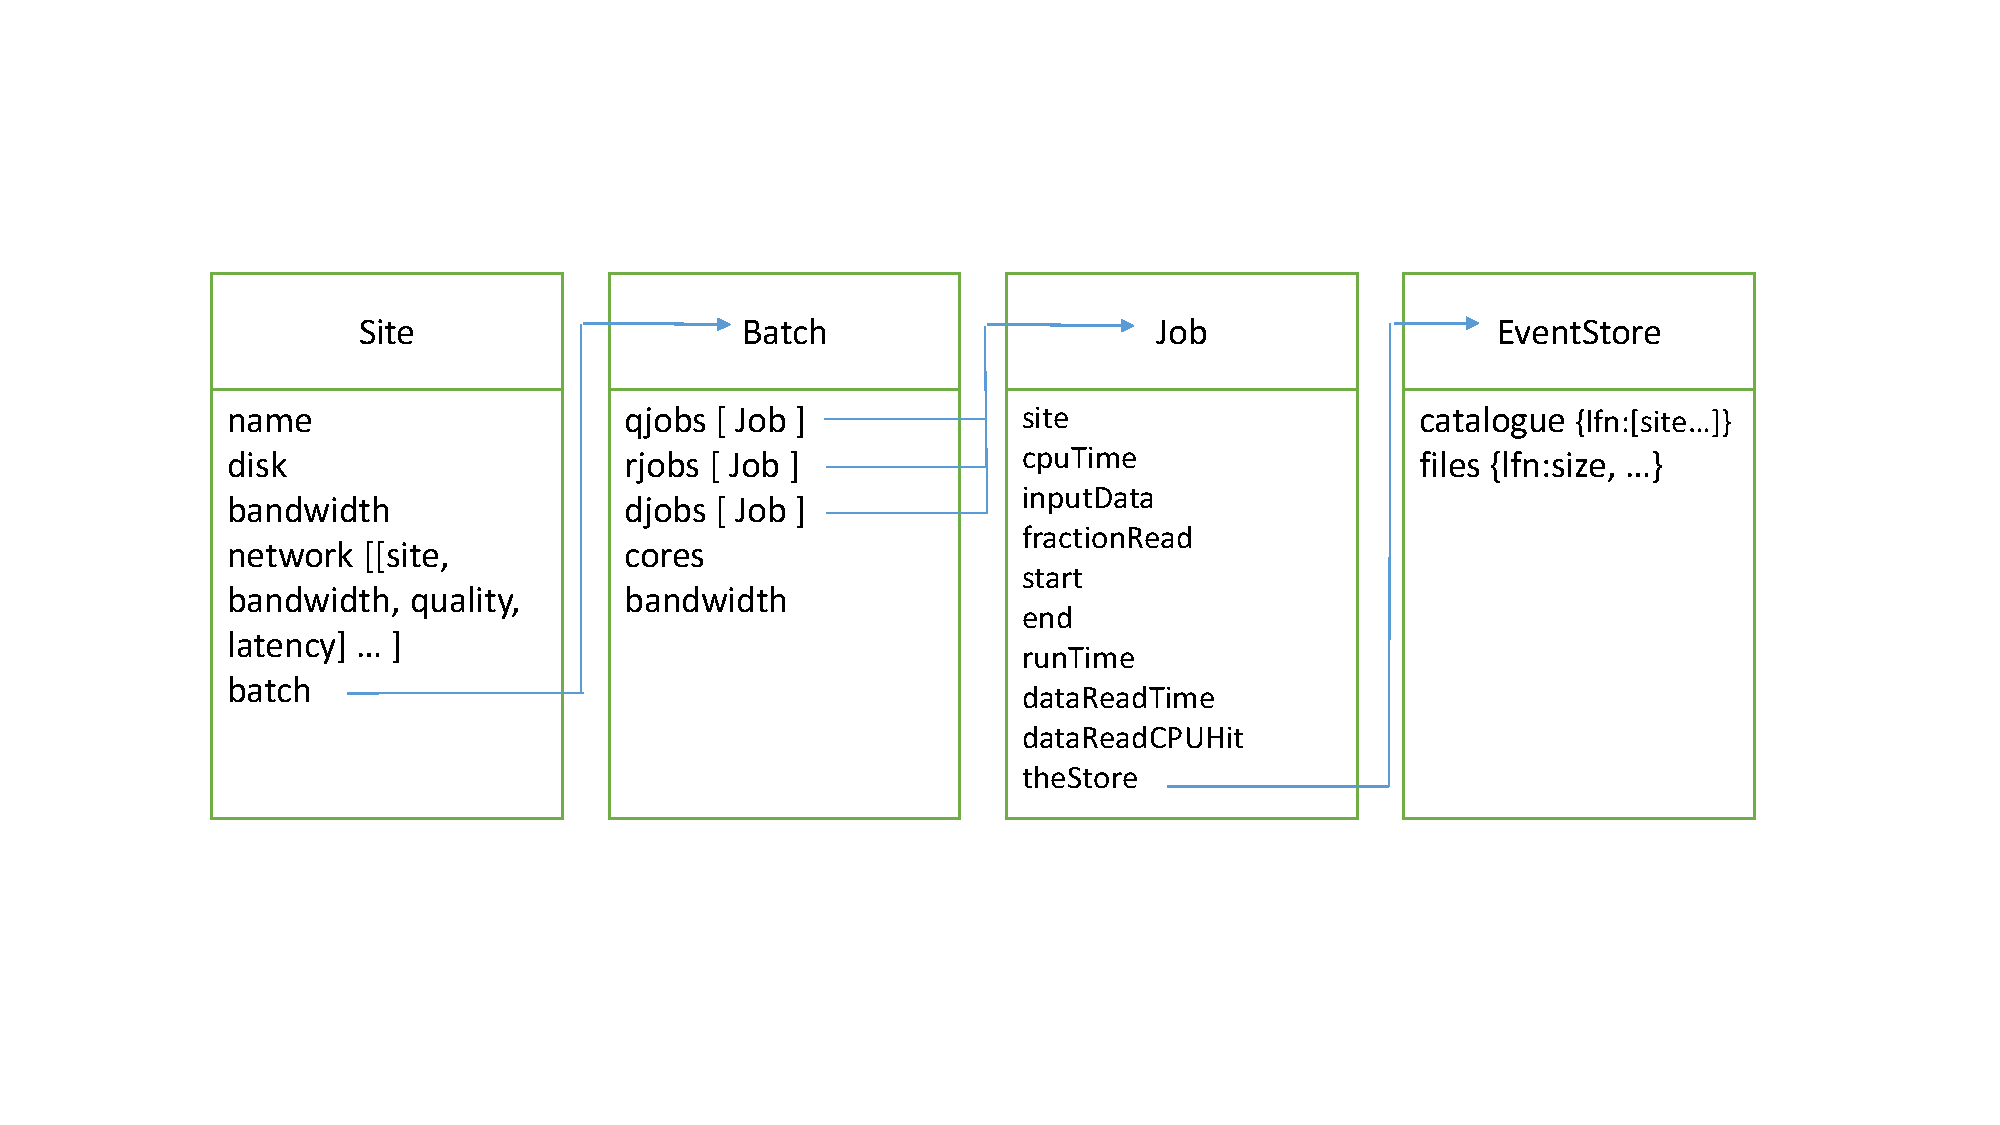
\includegraphics[trim=100 140 100 130, clip, width=\textwidth]{figures/classDiag.pdf}
  \caption{Software classes in the CMS Computing Model
    Simulation\label{fig:classDiag}}
\end{figure}

The batch system has a set of cores for running jobs. It also
contains, but doesn't currently use, a internal site bandwidth which
could further constrain the speed of jobs running at that site. It
maintains a list of jobs for each state, queued, running or done.

The disk storage system is configured as an available resource. Files
can be stored locally and use up this space. There is no tertiary data
storage system defined.

The network links to other sites are defined with information on the
bandwidth of the link, the latency implicit in that link and the quality
of the link. This information is used to determine how fast data will
flow over the links.

In addition there is also an Event Store that is used to define
information about files used in the system. It contains Logical File
Name (LFN) and size of each file. It also has knowledge of which sites
have files stored.

The information defined for a job is the CPU time required to carry it
out, the site it will run at, which LFNs it will read and what
fraction of that data it will read (currently defined to be 100\%). It
also remembers the original wall clock time required to run the job.

\subsection{Information Sources}

The simuation uses current system information to setup a complex and
realistic experiment wide computing system. Site information can be
extracted from the CMS
\htmladdnormallink{SiteDB}{http://cmsweb.cern.ch/sitedb/}
service. This provides information on the resources pledged to the
experiment for disk space and CPU power (defined in HEPSpec06). There
is an automated tool to extract this information (which was the most
recent 2014 pledges) and format it as input for the simulation. In
addition, when only considering the CMS infrastructure in the US these
numbers were extracted from
\htmladdnormallink{REBUS}{http://wlcg-rebus.cern.ch/apps/pledges/resources/}.

Once the sites are setup the links between them get setup then using
information extracted by a script from
\htmladdnormallink{PhEDEx}{http://cmsweb.cern.ch/phedex/}. 

\section*{References}
\begin{thebibliography}{9}
\bibitem{LHCMACHINE} Evans L and Bryant P,  LHC Machine {\it JINST}
  {\bf 3} S08001 (2008).

\bibitem{CMSDET} Chatrchyan S et al (CMS Collaboration),  The CMS
  experiment at the CERN LHC {\it JINST} {\bf 3} S08004 (2008).

\bibitem{CMSCTDR} Bayatyan G L et al,  CMS Computing Technical Design
  Report, CERN Report CERN-LHCC-2005-023 (2005).

\bibitem{HLLHC} Rossi L and Bruning O 2012 High Luminosity Large Hadron
  Collider - A description for the European Strategy Preparatory
  Group, CERN report CERN-ATS-2012-236

\bibitem{GAMEOVER} Fuller S H and Millet L I (Editors) 2011 {\it The
  Future of Computing Performance:  Game Over or Next Level?}
  The National Academies Press.

\bibitem{CHEP04BABAR} Brown D et. al. 2004 The new BaBar Analysis
  Model, {\it Proceedings of Computing in High Energy Physics (CHEP
    2004)}, Interlaken 

\bibitem{CM2CHEP04} Elmer P 2004 BaBar Computing - From Collisions to
  Physics Results, at Computing in High Energy and Physics (CHEP04)
  (Interlaken)

\bibitem{XROOTD1} Dorigo A, Elmer P, Furano F and Hanushevsky A 2005
  XROOTD - A highly scalable architecture for data access {\it WSEAS
    Transactions on Computers} {\bf 4.3 (2005)}

\bibitem{XROOTD2} Furano F, Elmer P, Hanushevsky A and Gerardo G 2006
  Latencies and Data Access. Boosting the performance of distributed
  applications {\it Proceedings of Computing in High Energy Physics
    (CHEP 2006)}, Mumbai

\bibitem{CHEP03PR} Ryd A, Crescente A, Dorigo A, Galeazzi F, Morandin
  M, Stroili R, Tiozzo G, Vedovato G, Tehrani F S, Pulliam T, Elmer P,
  Ceseracciu A, Piemontese M, Johnson D and Dasu S 2003 Distributed
  Offline Data Reconstruction in BaBar {\it proceedings of Computing
    in High Energy and Nuclear Physics (CHEP03)}, La Jolla
  [arXiv:cs/0306069 [cs.DC]]

\bibitem{AAACHEP13} Bloom K et al (CMS Collaboration) 2013 CMS Use of
  a Data Federation, submitted to proceedings of 20th International
  Conference on Computing in High Energy and Nuclear Physics (CHEP13),
  Amsterdam

\bibitem{PHEDEX} Rehn J et al 2006 PhEDEx high-throughput data
  transfer management system {\it Proceedings of Computing in High
    Energy Physics (CHEP 2006)}, Mumbai

\bibitem{SMSTORAGE} Butler M, Mount R and Hildreth M 2013 Snowmass
  2013 Computing Frontier Storage and Data Management
  [arXiv:1311.4580]

\bibitem{SMPROC} Elmer P, Rappoccio S, Stenson K and Wittich P 2013
  The Need for an R\&D and Upgrade Program for CMS Software and
  Computing [arXiv:1308.1247]

\bibitem{SMEFCOMP} Fisk I and Shank J 2013 Computing for the Energy
  Frontier: Snowmass Study 2013 [arXiv:1401.1840]

\bibitem{MAPREDUCE} Dean J and Ghemawat S 2004 MapReduce: Simplified Data Processing on Large Clusters, OSDI'04: Sixth Symposium on Operating System Design
and Implementation, San Francisco

\bibitem{ROOT} \url{http://root.cern.ch}

%\bibitem{iopartnum} IOP Publishing is to grateful Mark A Caprio, Center for Theoretical Physics, Yale University, for permission to include the {\tt iopart-num} \BibTeX package (version 2.0, December 21, 2006) with  this documentation. Updates and new releases of {\tt iopart-num} can be found on \verb"www.ctan.org" (CTAN).
\end{thebibliography}

\end{document}


